\section*{Tema 1}

\setcounter{problem}{0}

\begin{problem}
Fie \(J\) o mulțime arbitrară și \(c_j \in \complex\), \(\forall j \in J\). Arătați că:

\begin{enumerate}[a)]
    \item \(\displaystyle \sum_{j \, \in \, J} c_j\) este convergentă dacă și numai dacă \(\displaystyle \sum_{j \, \in \, J} \real c_j\) și \(\displaystyle \sum_{j \, \in \, J} \imag c_j\) sunt convergente.

    \item \(\displaystyle \sum_{j \, \in \, J} c_j\) este convergentă dacă și numai dacă \(\displaystyle \sum_{j \, \in \, J} \abs{c_j}\) este convergentă.
    
    \item Dacă \(\displaystyle \sum_{j \, \in \, J} c_j\) este convergentă, atunci mulțimea \(J_0 = \Set{ j \in J | c_j \neq 0 }\) este cel mult numărabilă.
\end{enumerate}
\end{problem}
\begin{solution}
Reamintim că \(\sum_{j \in J} c_j\) este \emph{convergentă} (sau \emph{sumabilă}) la \(S \in \complex\) dacă, pentru orice \(\varepsilon > 0\), există o mulțime finită de indici \(J_\varepsilon \subset J\), cu proprietatea că oricare ar fi o altă mulțime finită \(I\) cu \(J_\varepsilon \subset I \subset J\), avem \(\abs{\left(\sum_{i \in I} c_i\right) - S} < \varepsilon\).

\begin{enumerate}[a)]
    \item \begin{itemize}
        \item[\(\implies\)] Fie \(\Set{ c_j }\) un șir convergent. Pentru orice \(\varepsilon > 0\), luăm \(J_\varepsilon\) ca în definiția de mai sus. Asta înseamnă că \(\sum_{j \in J_\varepsilon} c_j\) este în interiorul bilei de centru \(S\) și rază \(\varepsilon\), și că orice număr finit de elemente din șir am mai adăuga, nu vom ieși din ea.
        
        Proiectând pe axa reală (respectiv pe cea imaginară), obținem că \(\sum_{j \in J_\varepsilon} \real c_j\) (respectiv \(\sum_{j \in J_\varepsilon} \imag c_j\)) este în interiorul bilei de centru \(\real S\) (respectiv \(\imag S\)) și rază \(\varepsilon\). Analog, orice număr finit de părți reale (respectiv părți imaginare) de elemente din șir am mai adăuga, nu vom ieși din aceste bile.
        
        \item[\(\impliedby\)] Vom nota \(S^{\real} \coloneq \sum_{j \in J} \real c_j\) și \(S^{\imag} \coloneq \sum_{j \in J} \imag c_j\) (acestea sunt numere reale, deoarece șirurile sunt convergente). Afirmăm că
        \[
            \sum_{j \in J} c_j = S \coloneq S^{\real} + i \, S^{\imag}
        \]
        
        Într-adevăr, pe baza definiției convergenței, obținem că pentru orice \(\varepsilon > 0\) putem găsi două mulțimi de indici \(J_\varepsilon^{\real}\) și \(J_\varepsilon^{\imag}\), astfel încât șirurile părților reale (respectiv imaginare) să fie la distanță cel mult \(\varepsilon\) de \(S^{\real}\) (respectiv \(S^{\imag}\)).
        
        Luând reuniunea \(J_\varepsilon \coloneq J_\varepsilon \cup J_\varepsilon\), care este tot o mulțime finită, putem deduce că \(\sum_{j \in J_\varepsilon} c_j\) se află în interiorul pătratului de centru \(S\) și latură \(\varepsilon\). Dar acest pătrat este conținut în cercul circumscris, de rază \(\frac{\sqrt{2}}{2} \varepsilon\).
        
        Notând această nouă valoare cu \(\varepsilon'\), observăm că poate fi făcută oricât de mică dorim, satisfăcând astfel condiția din definiția convergenței.
    \end{itemize}
    
    \item \begin{itemize}
        \item[\(\implies\)] Folosindu-ne de subpunctul anterior, și de faptul că șirurile \(\Set{ \real c_j }\) și \(\Set{ \imag c_j }\) sunt șiruri de numere reale, este suficient să arătăm că \(\sum_{j \in J} r_j\) convergentă implică \(\sum_{j \in J} \abs{r_j}\) convergentă, cu \(r_j \in \reals\).

        Să presupunem că \(\sum_{j \in J} r_j\) converge, dar \(\sum_{j \in J} \abs{r_j}\) nu. Vom nota cu \(\Set{ p_j }\) șirul termenilor \(\geq 0\) din \(r_j\) și cu \(\Set{ n_j }\) șirul termenilor strict negativi din \(r_j\) (unul dintre aceste șiruri ar putea fi și vid).
        
        Dacă ambele subșiruri sunt convergente, din faptul că \(\abs{p_j} = p_j\) și \(\abs{n_j} = - n_j\), am obține că \(\sum_{j \in J} \abs{c_j}\) este convergent și că
        \[
            \sum_{j \in J} \abs{c_j} = \sum_{j \in J} p_j - \sum_{j \in J} n_j,
        \]
        o contradicție cu ipoteza noastră că acest șir nu converge.
        
        Să presupunem, fără pierderea generalități, că \(\sum_{j \in J} p_j\) ar fi divergent. Atunci, există un indice \(j_1\) astfel încât
        \[
            p_1 + p_2 + \dots + p_{j_1} \geq 1
        \]
        Deoarece \(q_1 < 0\), avem că
        \[
            p_1 + p_2 + \dots + p_{j_1} - q_1 \geq 1
        \]
        Tot din divergență, rezultă că există un indice \(j_2\) astfel încât
        \[
            p_1 + \dots + p_{j_1} - q_1 + p_{j_1 + 1} + \dots + p_{j_2} - q_2 \geq 2
        \]
        și așa mai departe. Putem obține astfel că șirul inițial \(\sum_{j \in J} c_j\) nu este convergent, o contradicție cu ipoteza.

        \item[\(\impliedby\)] Știm că \(\sum_{j \in J} \abs{c_j}\) este convergentă.
        
        Fie \(\varepsilon_1 > 0\). Alegem \(J_{\varepsilon_1}\) ca în definiția convergenței pentru șirul \(\Set{ \abs{c_j} }\). Notăm \(z_1 \coloneq S_1 \coloneq \sum_{j \in J_{\varepsilon_1}} c_j\), care cu siguranță este un număr finit.
        
        Luând \(\varepsilon_2 = \varepsilon_1/2\), obținem un \(J_{\varepsilon_2}\) și un \(S_2\). Dacă considerăm \(J_{\varepsilon_1} \cup J_{\varepsilon_2}\), atunci știm că \(z_2 \coloneq \sum_{j \, \in \, J_{\varepsilon_1} \, \cup \, J_{\varepsilon_2}} c_j\) este la distanță cel mult \(\varepsilon_1\) de \(S_1\), dar și la distanță cel mult \(\varepsilon_2\) de \(S_2\). 
        
        Repetând construcția, obținem șirul \(S_1, S_2, \dots, S_n, \dots\) care este un șir Cauchy. Deoarece \(\complex\) este un spațiu metric complet, acest șir este convergent.
    \end{itemize}
    
    \item Fie \(\sum_{j \in J} c_j\) o serie convergentă. Din subpunctul anterior știm că și seria
    \[
        \sum_{j \in J} \abs{c_j}
    \]
    este la rândul ei convergentă. Vom nota valoarea acesteia cu \(S\).
    
    Definim mulțimile
    \[
        J_n = \Set{ j \in J | \abs{c_j} > \frac{1}{n} }
    \]
    pentru orice \(n \in \naturals^*\).
    
    Afirmăm că fiecare \(J_n\) este finită. Altfel, dacă ar exista un \(k \in \naturals^*\) astfel încât \(J_k\) să fie infinită, pentru orice \(\varepsilon > 0\) am putea adăuga la mulțimea \(J_\varepsilon\) un număr de \(\ceil{\varepsilon \cdot k}\) elemente de normă \(\frac{1}{k}\), iar asta ar contrazice definiția convergenței.

    Luând reuniunea mulțimilor \(J_n\) după toate valorile lui \(n \in \naturals\), obținem exact mulțimea \(J_0\). Dar o reuniune numărabilă de mulțimi finite este cel mult numărabilă, ceea ce era de demonstrat.
\end{enumerate}
\end{solution}

\begin{problem}
Fie \(f \in \sheaf(\complex^n)\). Presupunem că există \(\nu \in \naturals^n\) și \(C > 0\) astfel încât pentru orice \(z \in \complex^n\) avem \(\abs{f(z)} \leq C \, \abs{ \, z^\nu \, }\). Arătați că \(f\) este funcție polinomială.
\end{problem}
% TODO: solve

\begin{problem}
Fie \(\Omega\) un deschis conex din \(\complex^n\) și \(f_1, \dots, f_k \in \sheaf(\Omega)\). Dacă funcția \(\sum_{j = 1}^{k} \abs{ \, f_j \, }^2\) este constantă, arătați că toate funcțiile \(f_j\) sunt constante.
\end{problem}
\begin{solution}
De obicei, atunci când vrem să arătăm că o funcție derivabilă este constantă, îi calculăm derivata și arătăm că aceasta este 0 (sau că toate derivatele parțiale sunt 0, în cazul multivariat).

Știm din ipoteză că funcția \(\sum_{j = 1}^{k} \abs{ \, f_j \, }^2\) este constantă, deci derivata ei în raport cu orice variabilă va fi 0. În cazul nostru, identitatea \(\abs{\, f \,}^2 = f \cdot \overline{f}\) ne duce cu gândul la derivarea în raport cu \(z_i\) și cu \(\overline{z}_i\), pentru orice \(i \in \Set{1, \dots, n}\) fixat.

Avem că:
\begin{align*}
    \frac{\partial}{\partial z_i} \frac{\partial}{\partial \, \overline{z}_i} \left(\, \sum_{j = 1}^{k} \abs{ \, f_j \, }^2\right) &=
    \sum_{j = 1}^{k} \frac{\partial}{\partial z_i} \frac{\partial}{\partial \, \overline{z}_i} \left(f_j \cdot \overline{f_j}\right) = \\
    &= \sum_{j = 1}^{k} \frac{\partial}{\partial z_i} \left(\underbrace{\frac{\partial f_j}{\partial \, \overline{z}_i}}_{= \, 0} \cdot \overline{f_j} + f_j \cdot \frac{\partial \overline{f_j}}{\partial \, \overline{z}_i}\right) = \\
    &= \sum_{j = 1}^{k} \frac{\partial}{\partial z_i} \left(f_j \cdot \overline{\left(\frac{\partial f_j}{\partial z_i}\right)}\right) = \\
    &= \sum_{j = 1}^{k} \left(\frac{\partial f_j}{\partial z_i} \cdot \overline{\left(\frac{\partial f_j}{\partial z_i}\right)} + f_j \cdot \underbrace{\frac{\partial}{\partial z_i} \overline{\left(\frac{\partial f_j}{\partial z_i}\right)}}_{= \, 0}\right) = \\
    &= \sum_{j = 1}^{k} \frac{\partial f_j}{\partial z_i} \cdot \overline{\left(\frac{\partial f_j}{\partial z_i}\right)}
    = \sum_{j = 1}^{k} \, \abs{\frac{\partial f_j}{\partial z_i}}^2
\end{align*}
În calcule, ne-am folosit de faptul că derivata parțială a unei funcții olomorfe în raport cu \(\overline{z}_i\) (respectiv a unei funcții antiolomorfe în raport cu \(z_i\)) este întotdeauna zero.

Evaluând expresia de mai sus într-un punct \(w \in \Omega\), obținem că
\[
    \sum_{j = 1}^{k} \abs{\frac{\partial f_j}{\partial z_i} (w)}^2 = 0, \enspace \forall i = \overline{1, n}
\]
Fiind o sumă de numere reale pozitive, singura posibilitate este 
\[
    \frac{\partial f_j}{\partial z_i} = 0, \enspace \forall i, j = \overline{1, n}
\]
De aici rezultă că toate funcțiile \(f_j\) sunt constante, toate derivatele lor parțiale fiind zero.
\end{solution}

\begin{comment}
\begin{problem}
Arătați că \(\complex^2 \setminus \Set{ (n, 0) | n \in \naturals }\) nu este biolomorfă cu \(\complex^2 \setminus \left(\Set{ \frac{1}{n} | n \in \naturals^* } \cup \Set{0}\right)\).
\end{problem}
\end{comment}

\begin{comment}
\begin{problem}
Fie \(\Omega \subset \complex^2\) definit prin
\[
    \Omega = \Set{ (z_1, z_2) \in \complex^2 | \abs{\, z_1 (1 - z_2)^2 } + \abs{\, z_2 \,}^2 < 1 }
\]
\begin{enumerate}[a)]
    \item Arătați că \(\Omega\) nu este mărginit.

    \item Arătați că \(\Omega\) este biolomorf cu bila unitate
    \[
        B = \Set{ (z_1, z_2) \in \complex^2 | \abs{z_1}^2 + \abs{z_2}^2 < 1 }
    \]

    \item Arătați că \(\partial \Omega\) conține o subvarietate complexă închisă a lui \(\complex^2\), de dimensiune 1.
    
    \item Arătați că dacă \(U\) este un deschis din \(\complex^n\) și \(U \supset \overline{\Omega}\), atunci \(U\) nu poate fi biolomorf cu \(B\).
    
    \item Arătați că nu există un deschis \(U\) din \(\complex^2\) și o subvarietate închisă \(L\) a lui \(U\) astfel încât \(\dim L = 1\) și \(L\) să fie inclusă în frontiera bilei \(B\).
\end{enumerate}
\end{problem}
\end{comment}

\begin{problem}
Fie \(M\) o varietate complexă și \(x, y \in M\) două puncte. Dacă \(\holomorphichull[M]{\Set{x}} \cap \holomorphichull[M]{\Set{y}} \neq \emptyset\), atunci arătați că \(\holomorphichull[M]{\Set{x}} = \holomorphichull[M]{\Set{y}}\).
\end{problem}
\begin{solution}
Fie \(z \in \holomorphichull[M]{\Set{x}}\). Vom arăta că \(\holomorphichull[M]{\Set{z}} = \holomorphichull[M]{\Set{x}}\).

Începem prin a scrie definiția pentru acoperirea olomorf convexă a lui \(\Set{x}\):
\begin{align*}
    \holomorphichull[M]{\Set{x}} &= \Set{ p \in M | \abs{f(p)} \leq \norm{f}_{\Set{x}}, \forall f \in \sheaf(M) } \\
    &= \Set{ p \in M | \abs{f(p)} \leq \abs{f(x)}, \forall f \in \sheaf(M) }
\end{align*}
În particular, deoarece \(z \in \holomorphichull[M]{\Set{x}}\), știm că \(\abs{f(z)} \leq \abs{f(x)}\), \(\forall f \in \sheaf(M)\). Asta demonstrează că \(\holomorphichull[M]{\Set{z}} \subseteq \holomorphichull[M]{\Set{x}}\).

Pentru cealaltă implicație, fie \(p \in \holomorphichull[M]{\Set{x}}\). Folosindu-ne de observația de mai sus, știm că \(\abs{f(p)} \leq \abs{f(x)}\) pentru orice \(f \in \sheaf(M)\). Vrem să arătăm că \(p \in \holomorphichull[M]{\Set{z}}\), sau cu alte cuvinte, că \(\abs{f(p)} \leq \abs{f(z)}\) pentru orice funcție olomorfă \(f\).

Să presupunem că există \(f \in \sheaf(M)\) astfel încât \(\abs{f(p)} > \abs{f(z)}\). Folosindu-ne de faptul că \(z\) este în acoperirea olomorfă a lui \(\Set{x}\), obținem inegalitatea
\[
    0 \leq \abs{f(z)} < \abs{f(p)} \leq \abs{f(x)}
\]
Înlocuind \(f\) cu \(g \coloneq f - f(x)\) (tot o funcție olomorfă), obținem
\[
    0 \leq \abs{f(z) - f(x)} < \abs{f(p) - f(x)} < \abs{f(x) - f(x)} = 0
\]
care este o contradicție.
\end{solution}

\begin{comment}
\begin{problem}
Dați exemplu de o varietate complexă \(M\), un deschis relativ compact \(B\) în \(M\) și un punct \(a \in M\) astfel încât:
\begin{itemize}
    \item \(B\) este biolomorf cu o bilă din \(\complex^n\), unde \(n\) este dimensiunea lui \(M\),
    \item \(\overline{B}\) este olomorf convex în \(M\),
    \item \(\overline{B} \cup \Set{a}\) nu este olomorf convex în \(M\).
\end{itemize}
\end{problem}
\end{comment}

\setcounter{problem}{7}

\begin{problem}
~
\begin{enumerate}[a)]
    \item Dacă \(M\) este o varietate complexă și \(\Set{ K_n }_{n \in \naturals}\) este un șir de compacți din \(M\) astfel încât \(K_n \supseteq K_{n + 1}\) pentru orice \(n\), iar \(K \coloneq \bigcap_{n \in \naturals} K_n\), atunci \(\bigcap_{n \in \naturals} \holomorphichull{K_n} = \holomorphichull{K}\).
    
    \item Dați exemplu de o varietate complexă \(M\) și un șir de compacți din \(M\), \(\Set{ K_n }_{n \in \naturals}\), astfel încât \(\bigcap_{n \in \naturals} \holomorphichull{K_n} \neq \holomorphichull{K}\).
\end{enumerate}
\end{problem}
\begin{solution}
\begin{enumerate}[a)]
    \item Vom demonstra egalitatea de mulțimi prin dublă incluziune.
    
    % TODO: reasoning might be wrong
    
    \begin{itemize}
        \item[\(\subseteq\)] Fie \(x \in \bigcap_{n \in \naturals} \holomorphichull{K_n}\). Asta înseamnă că \(x \in \holomorphichull{K_n}\), \(\forall n \in \naturals\).
        
        Fie \(f \in \sheaf(M)\) fixat. Folosind definiția acoperirii olomorf convexe, obținem că
        \[
            \abs{f(x)} \leq \norm{f}_{K_n}
        \]
        pentru orice \(n\). În particular, \(\abs{f(x)}\) este o margine inferioară pentru \(\Set{ \norm{f}_{K_n} }\).
        
        Din ipoteză știm că
        \[
            \dots \supseteq K_{n - 1} \supseteq K_n \supseteq K_{n + 1} \supseteq \dots
        \]
        de unde
        \[
            \dots \geq \norm{f}_{K_{n - 1}} \geq \norm{f}_{K_n} \geq \norm{f}_{K_{n + 1}} \geq \dots
        \]
        deoarece valoarea maximă a lui \(f\) pe o submulțime nu poate depăși valoarea maximă pe mulțimea care o conține.
        
        Folosindu-ne de proprietățile maximului, avem că
        \[
            \norm{f}_K = \inf_{n \in \naturals} \Set{ \norm{f}_{K_n} }
        \]
        Deoarece infimumul este cea mai mare margine inferioară, rezultă că \(\abs{f(x)} \leq \norm{f}_K\). Cu alte cuvinte, \(x \in \holomorphichull{K}\).
        
        \item[\(\supseteq\)] Fie \(x \in \holomorphichull{K}\). Atunci, pentru orice \(f \in \sheaf(M)\), avem că
        \[
            \abs{f(x)} \leq \norm{f}_K = \max_{z \in K} \, \abs{f(z)}
        \]
        
        Deoarece \(K \subseteq K_n\) pentru orice \(n\), știm sigur că
        \[
            \max_{z \in K} \, \abs{f(z)} \leq \max_{z \in K_n} \abs{f(z)} = \norm{f}_{K_n},
        \]
        de unde rezultă că \(x \in \holomorphichull{K_n}\), pentru orice \(n\). Luând intersecția, obținem \(x \in \bigcap_{n \in \naturals} \holomorphichull{K_n}\).
    \end{itemize}
    
    \item Observăm că în demonstrația de mai sus nu am avut nevoie de ipoteza adițională \(K_n \supseteq K_{n + 1}\) pentru a demonstra incluziunea ``\(\supseteq\)''. Deci vom căuta un contraexemplu pentru care \(\bigcap \holomorphichull{K_n} \not\subseteq \holomorphichull{K}\).
    
    Vom lua cercul unitate \(S^1 \subset \complex\) și un șir de elipse imbricate, cu semiaxa mică din ce în ce mai scurtă. Această situație este descrisă în figura \ref{hw1-pb8}.
    
    \begin{figure}[htbp]
        \centering
        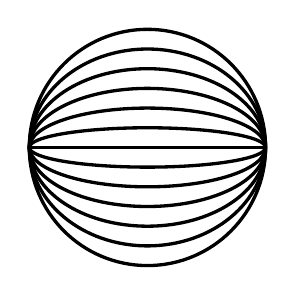
\begin{tikzpicture}
            \draw[black, very thick](0,0) circle (1.5);
            \draw[black, very thick](0,0) ellipse (1.5 and 1.25);
            \draw[black, very thick](0,0) ellipse (1.5 and 1);
            \draw[black, very thick](0,0) ellipse (1.5 and 0.75);
            \draw[black, very thick](0,0) ellipse (1.5 and 0.5);
            \draw[black, very thick](0,0) ellipse (1.5 and 0.25);
            \draw[black, very thick](0,0) ellipse (1.5 and 0);
        \end{tikzpicture}
        \caption{Un șir \(K_n\) de compacți în \(\complex\)}
        \label{hw1-pb8}
    \end{figure}
    
    În acest exemplu, \(K = \bigcap K_n = \Set{ \text{două puncte diametral opuse} }\), deci \(K = \holomorphichull{K}\), dar fiecare \(\holomorphichull{K_n}\) este un cerc sau o elipsă luată cu tot cu interiorul ei pentru orice \(n\), deci \(\bigcap{\holomorphichull{K_n}} = \Set{ \text{diametru de cerc} }\).
\end{enumerate}
\end{solution}

% TODO: solve remaining problems